\newcommand{\ClassPath}{../VIU_TFM_LaTeX_template}
\documentclass{\ClassPath/viu-tfm-template}
\usepackage{multicol}

\definecolor{maincolor}{HTML}{f25416}

%--------------------------------------------------------------------------
% Definiciones necesarias Modifica con tus datos
%--------------------------------------------------------------------------
\def\nombre{Gómez Olivencia, Rubén}
\def\dni{78910013-A}
\def\titulo{Despliegue de aplicaciones en AWS}
\def\subtitulo{(Beanstalk, Automatización con Gitlab y Terraform)}
\def\titulacion{Máster Universitario en Desarrollo de Aplicaciones y Servicios Web}
\def\curso{2022-2023}

%Los siguientes son opcionales: si no se ponen, la portada cambia un poco. Ideal para escribir artículos/trabajos cortos
\def\dirige{}
\def\codirige{}
\def\convocatoria{}
\def\asignatura{Computación en la nube}


% importar fichero de Bibliografía
%\addbibresource{Actividad_1.bib}

\begin{document}
    \graphicspath{{../VIU_TFM_LaTeX_template/}}

    \coverpage

    \tableofcontents

\chapter{Introducción}

A la hora de poner un proyecto en producción era habitual realizar el despliegue de manera manual, teniendo que realizar la instalación y la configuración de cada servicio que se vaya a necesitar.

A día de hoy el despliegue manual ha sufrido muchas mejoras gracias a los sistemas de contenedores, como ejemplo \href{https://www.docker.com/}{Docker} o sistemas PaaS (plataformas como servicio) como \href{https://en.wikipedia.org/wiki/AWS_Elastic_Beanstalk}{AWS Elastic Beanstalk}.

Por otro lado, tenemos la posibilidad de realizar despliegues automatizados gracias a los nuevos sistemas de integración continua y despliegue continuo (CI/CD), muy utilizado en la metodología DevOps. De esta manera, una vez creado el \textit{pipeline} de ejecución, el despliegue siempre se realizará de la misma manera.

Si al punto anterior le añadimos la creación de toda la infraestructura mediante código (IaC, \textit{Infraestructure as code}), pasar de un proveedor de servicios en la nube a otro se convierte en una tarea mucho más sencilla.

En este documento usaremos la aplicación \href{https://flarum.org/}{Flarum} como ejemplo para realizar los distintos despliegues explicados previamente.


\chapter{Base de datos RDS}
Para la aplicación se va a necesitar una base de datos, por lo que va a ser lo primero que se va a desplegar.

AWS permite realizar el despliegue de distintos gestores de bases de datos a través de su servicio \textbf{RDS} (\textit{Relational Database Service}). En este caso se va a desplegar un RDS de MySQL 5.X con las siguientes características:

\begin{itemize}
    \item RDS de tipo db.t3.micro
    \item Almacenamiento 20Gib SSD de uso general (gp2).
    \item Cifrado en reposo habilitado.
    \item Nombre bd = DB\_flarum
    \item User = admFlarum
    \item Password = Viu2022Flarum
    \item Charset = utf8mb4
    \item Collation = utf8mb4\_unicode\_ci
\end{itemize}

Es importante añadirle un grupo de seguridad que permita todo el tráfico entrante procedente de la red del VPC de AWS (por defecto 172.31.0.0/16).


\begin{center}
    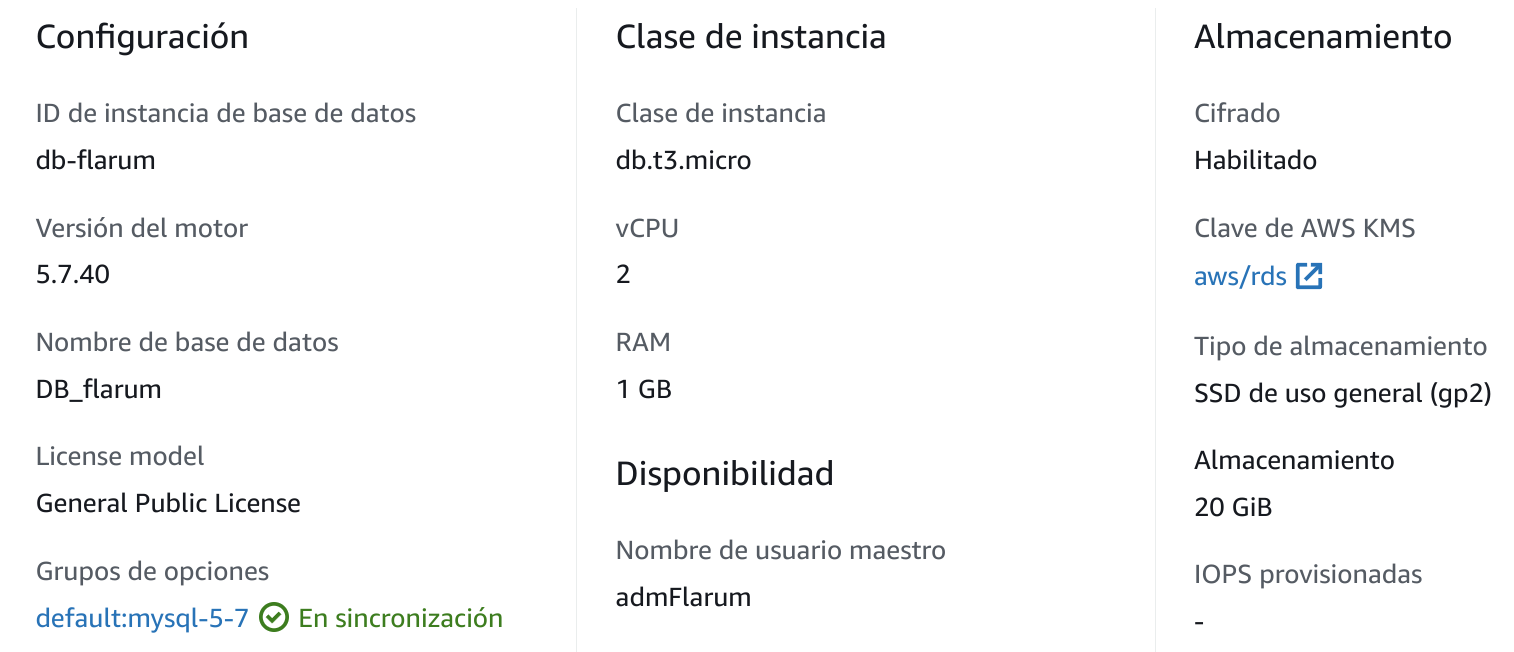
\includegraphics[frame,width=0.8\linewidth]{img/rds.png}
\end{center}

Con esto ya tendríamos creada la base de datos.


\chapter{Despliegue con AWS Elastic Beanstalk}

\href{https://aws.amazon.com/es/elasticbeanstalk/}{Amazon Elastic Beanstalk} nos permite crear y desplegar aplicaciones web de manera sencilla sin tener que realizar la tediosa configuración que hay detrás de ello, ya que lo hace de manera automática.

Para realizar el despliegue de Flarum se ha utilizado la siguiente configuración personalizada, a través del editor avanzado al crear el entorno de Beanstalk:
\vspace{-15pt}
\begin{itemize}
    \item \textbf{Nombre de la aplicación} = flarum
    \item \textbf{Nombre del entorno} = pro-rg-08masw
    \item Sin balanceador de carga.
    \item \textbf{Entorno}: PHP 8.0
    \item \textbf{Servidor Web} = apache
    \item \textbf{Raíz del documento}: /public
    \item \textbf{Mostrar errores}: On
    \item \textbf{Código fuente} de la aplicación obtenido del siguiente \href{https://amn-viu-resources-public.s3.eu-west-1.amazonaws.com/08masw/actividad2/flarum_php8.0.zip}{enlace}.
\end{itemize}

Tras crear el entorno, nos aparecerá a modo resumen en el interfaz lo siguiente:
\begin{center}
    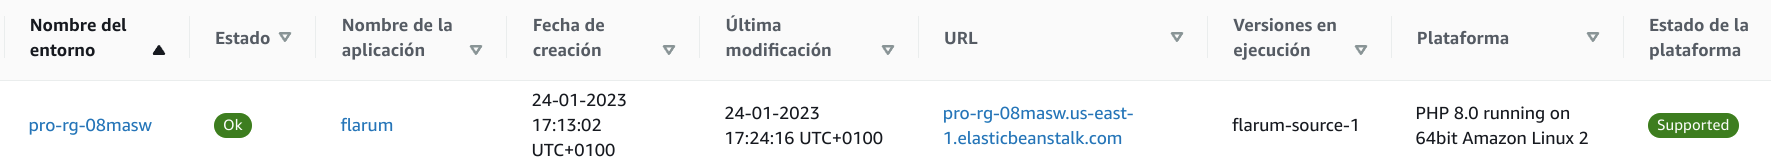
\includegraphics[frame,width=\linewidth]{img/beanstalk.png}
\end{center}

Para poder acceder al nuevo entorno a través del navegador web, vemos cómo se nos ha creado una URL propia \href{http://pro-rg-08masw.us-east-1.elasticbeanstalk.com/}{pro-rg-08masw.us-east-1.elasticbeanstalk.com}, que al acceder nos muestra el panel de configuración de Flarum:

\vspace{-10pt}
\begin{center}
    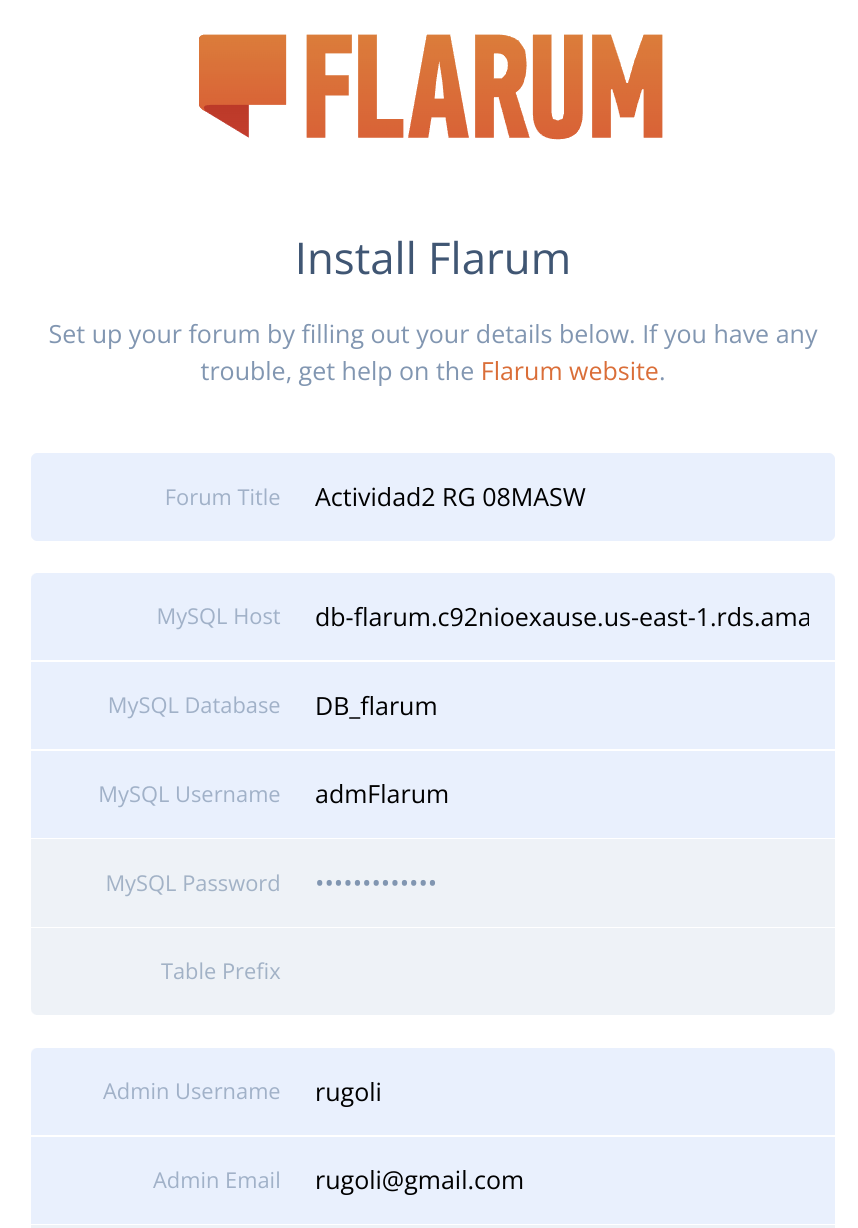
\includegraphics[frame,width=0.63\linewidth]{img/flarum-0.png}
\end{center}

En este formulario nos aparecen las opciones que debemos rellenar para que se acceda a la base de datos creada previamente. Tras introducir los datos de manera correcta, la aplicación desplegará las tablas que necesita y ya podremos acceder a la aplicación.

\begin{center}
    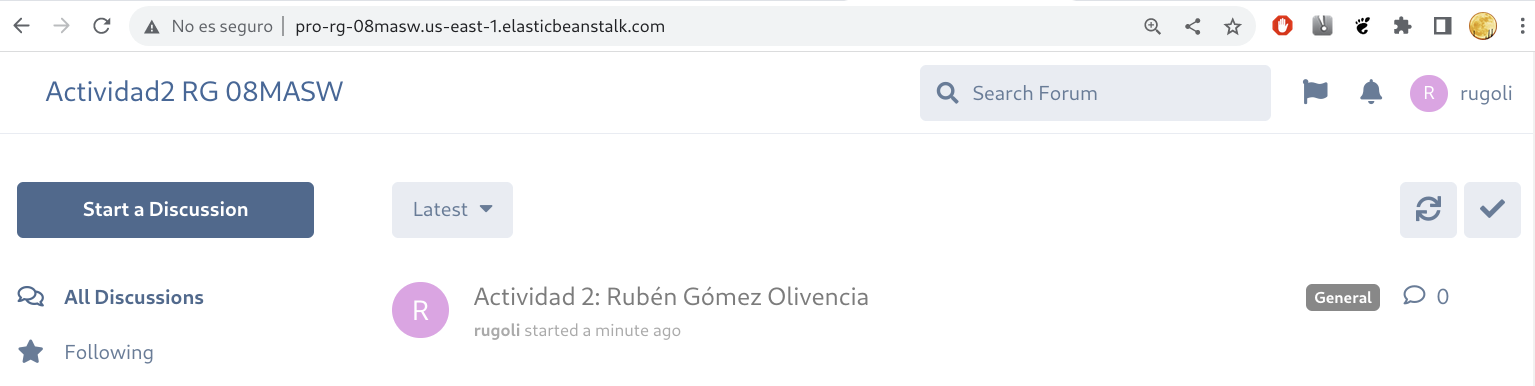
\includegraphics[frame,width=\linewidth]{img/flarum-1.png}
\end{center}

En la imagen superior se puede cómo se ha podido crear una nueva entrada en el foro recién desplegado.


\chapter{Despliegue automatizado desde GitLab}

Para este apartado vamos a utilizar \href{https://gitlab.com/}{GitLab} para realizar el despliegue de manera automatizada a través de su sistema de integración continua y despliegue continuo (CI/CD).

Lo primero que tenemos que hacer es crear un nuevo repositorio con el código obtenido de este \href{https://amn-viu-resources-public.s3.eu-west-1.amazonaws.com/08masw/actividad2/flarum_php8.0.zip}{enlace}.

\begin{center}
    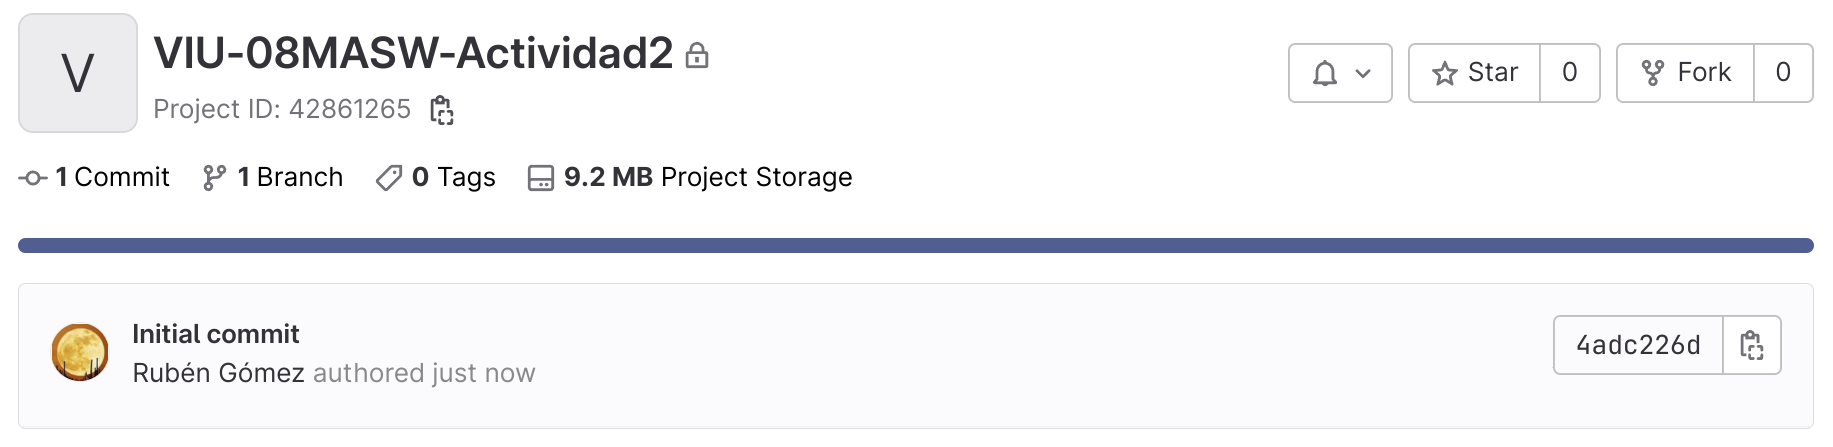
\includegraphics[frame,width=\linewidth]{img/gitlab.png}
\end{center}

Tras subir el código hay que realizar las siguientes modificaciones:

\begin{itemize}
    \item Añadir el fichero \configfile{.gitlab-ci.yml} :  Es el encargado de lanzar el \textit{pipeline}, que son las instrucciones para realizar el despliegue automatizado que ejecuta GitLab al recibir un commit del código en la rama \textbf{main}.
\end{itemize}
\begin{mycode}{Automatización con  .gitlab-ci.yml}{yaml}{{\scriptsize }}
image: "php:8.0"
stages:
  - build
  - deploy
cache:
  key: cache-key
  paths:
  - vendor/
  - node_modules/
before_script:
  - apt-get update
  - apt-get install -y python3 python3-pip wget zip unzip git
  - pip -V
.build:
  script:
    - echo "Building app"
    - apt-get install -y libpng-dev libxml2-dev libzip-dev sudo nodejs npm
    - wget https://composer.github.io/installer.sig -O - -q | tr -d '\n' > installer.sig
    - php -r "copy('https://getcomposer.org/installer', 'composer-setup.php');"
    - php composer-setup.php --install-dir=/usr/local/bin -filename=composer --version=2.0.14
    - php -r "unlink('composer-setup.php'); unlink('installer.sig');"
    # Extra PHP libraries
    - docker-php-ext-install gd
    - docker-php-ext-install soap
    - docker-php-ext-install zip
    - zip ../myapp.zip -r * .[^.]* >/dev/null
    - mv ../myapp.zip .
  artifacts:
    paths:
    - myapp.zip
    expire_in: 1 week
.deploy:
  script:
    - echo "Deploy in server"
    - pwd
    - ls -la
    # AWScli de ElasticBeanstalk
    - pip install awsebcli==3.18
    - export PATH=~/.local/bin:$PATH
    # Credentials AWS (Profile)
    - set -x
    - set -e
    - mkdir ~/.aws
    - touch ~/.aws/config
    - chmod 600 ~/.aws/config
    - echo "[profile eb-cli]" > ~/.aws/config
    - echo "aws_access_key_id=$AWS_ACCESS_KEY_ID" >> ~/.aws/config
    - echo "aws_secret_access_key=$AWS_SECRET_ACCESS_KEY" >> ~/.aws/config
    - echo "aws_session_token=$AWS_SESSION_TOKEN_KEY" >> ~/.aws/config
    # Deploy
    - cp $CONFIG_FILE_BEAN_STALK_AWS .elasticbeanstalk/config.yml
    - eb --version
    - eb status --verbose $ENV_BEAN_STALK_AWS
    - eb use $ENV_BEAN_STALK_AWS
    - eb deploy
1_build_pro:
  extends: .build
  stage: build
  only:
    - main

2_deploy_pro:
  extends: .deploy
  stage: deploy
  variables:
    ENV_BEAN_STALK_AWS: "pro-rg-08masw"
    CONFIG_FILE_BEAN_STALK_AWS: ".elasticbeanstalk/config.pro.yml"
  only:
  - main\end{mycode}

\begin{itemize}
    \item Modificar el fichero \configfile{.elasticbeanstalk/config.pro.yml} para que el \textit{pipeline} anterior lo utilice para realizar el despliegue. El despliegue se realizará sobre el mismo Beanstalk creado previamente.

    \begin{mycode}{Fichero de configuración para Beanstalk}{yaml}{}
global:
  application_name: flarum
  default_ec2_keyname: null
  default_region: us-east-1
  include_git_submodules: true
  instance_profile: null
  platform_name: null
  platform_version: null
  profile: eb-cli
  sc: git
  workspace_type: Application
deploy:
  artifact: ./myapp.zip\end{mycode}

    \item Añadir \textbf{variables} de entorno dentro del repositorio GitLab (en \textit{Settings → CI/CD → Variables}). El valor de estas variables será sustituido dentro del pipeline. De esta manera no introducimos credenciales en el código fuente del repositorio.
    \begin{center}
        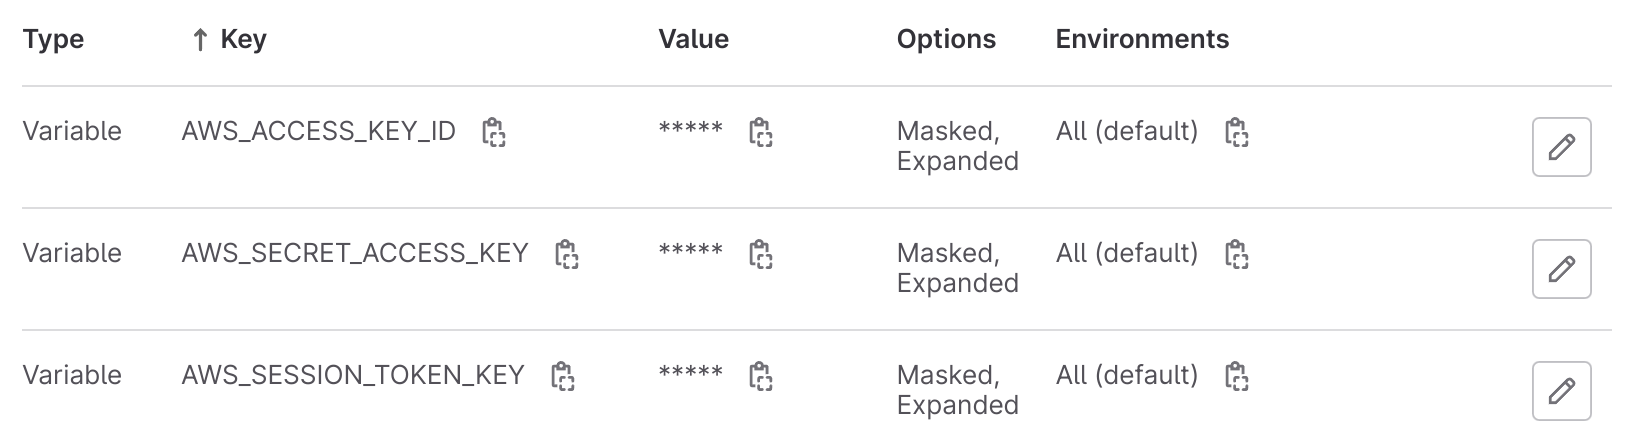
\includegraphics[frame,width=\linewidth]{img/gitlab-vars.png}
    \end{center}
\end{itemize}

Una vez realizadas las modificaciones, el \textit{pipeline} se ejecutará, y tras esperar a que termine los dos pasos del despliegue, en GitLab veremos un resumen:

\begin{center}
    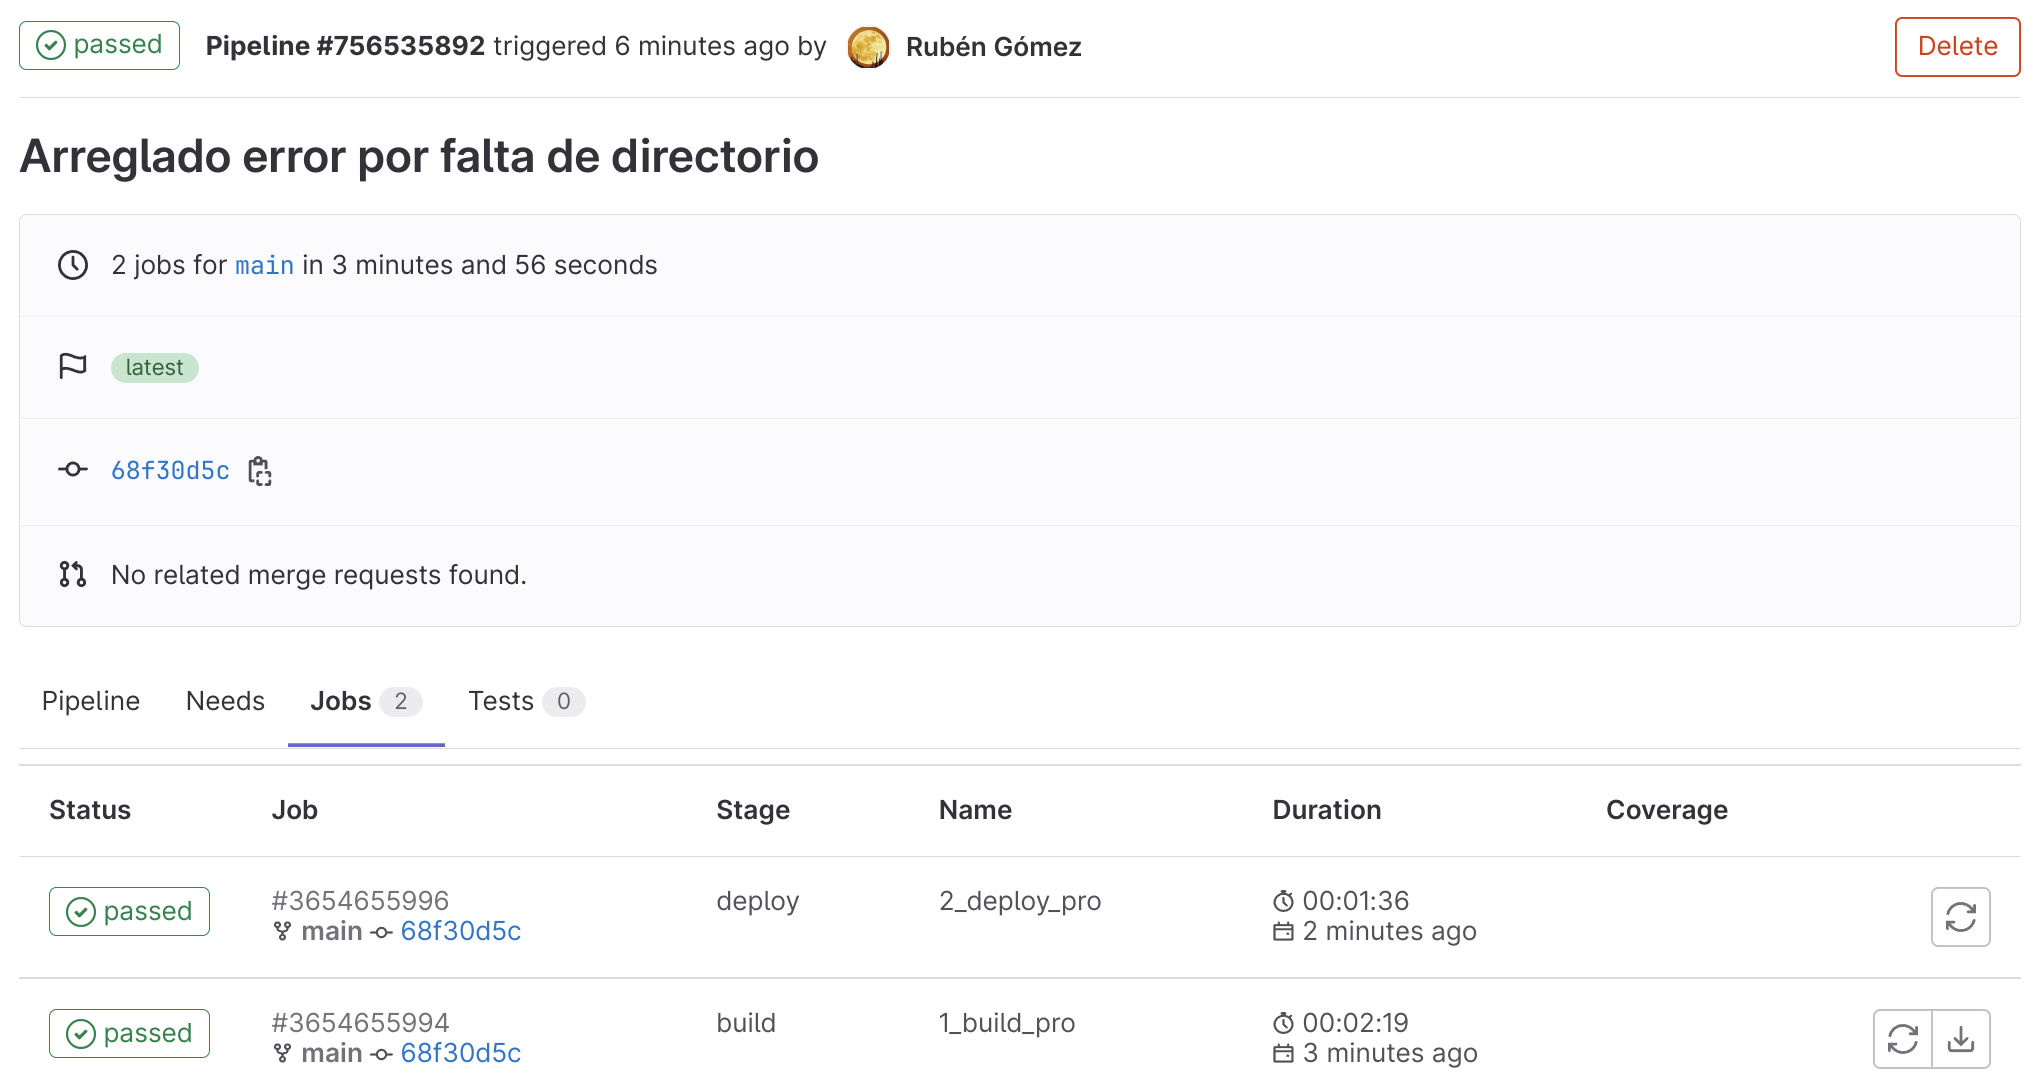
\includegraphics[frame,width=\linewidth]{img/gitlab-pipeline.png}
\end{center}

Beanstalk necesita del código fuente de la aplicación para realizar el despliegue. Este se ha subido a través del \textbf{\textit{artifact}} que se ha creado en el \textit{pipeline} (“myapp.zip”), que en AWS se añade dentro de un bucket S3 creado específicamente para Beanstalk.

A continuación se puede ver cómo se han subido varios ficheros tras realizar distintos despliegues:
\begin{center}
    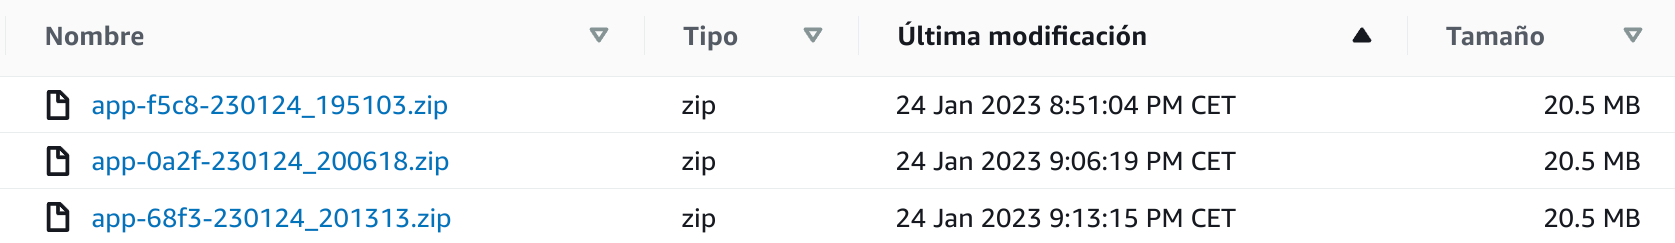
\includegraphics[frame,width=\linewidth]{img/s3.png}
\end{center}

Dado que es un sistema automatizado, deberíamos también controlar el número de ficheros que se tienen en el bucket S3 para no incurrir en gastos innecesarios.

Tras realizar el despliegue, al ir a la URL proporcionada por Beanstalk,  nos aparecerá el asistente de configuración de Flarum, en el que debemos volver a añadir la configuración necesaria. Si utilizamos la misma base de datos del despliegue anterior dará un error, por lo que es importante acordarnos de borrar las tablas existentes.

\begin{center}
    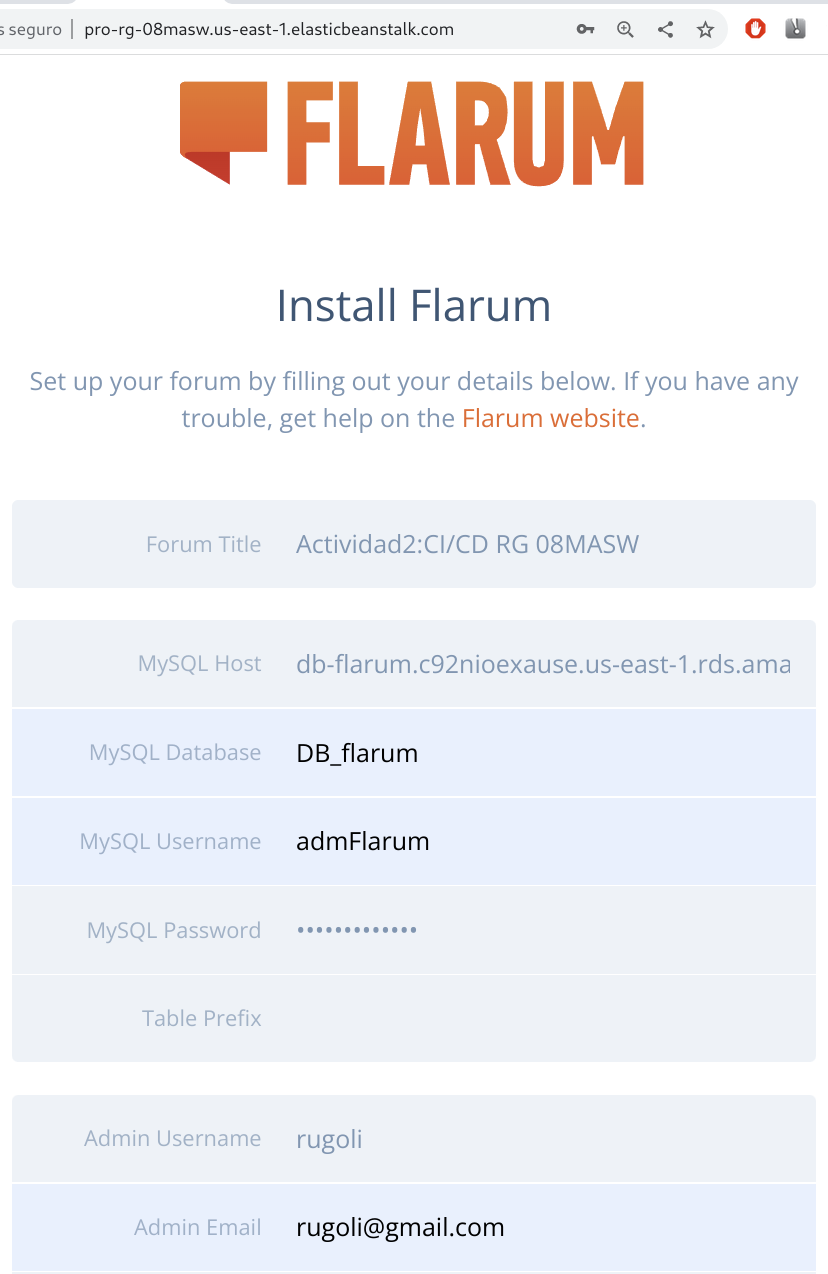
\includegraphics[frame,width=0.63\linewidth]{img/flarum-2.png}
\end{center}

Después de la creación de las tablas y el despliegue inicial, ya podremos utilizar la aplicación:
\begin{center}
    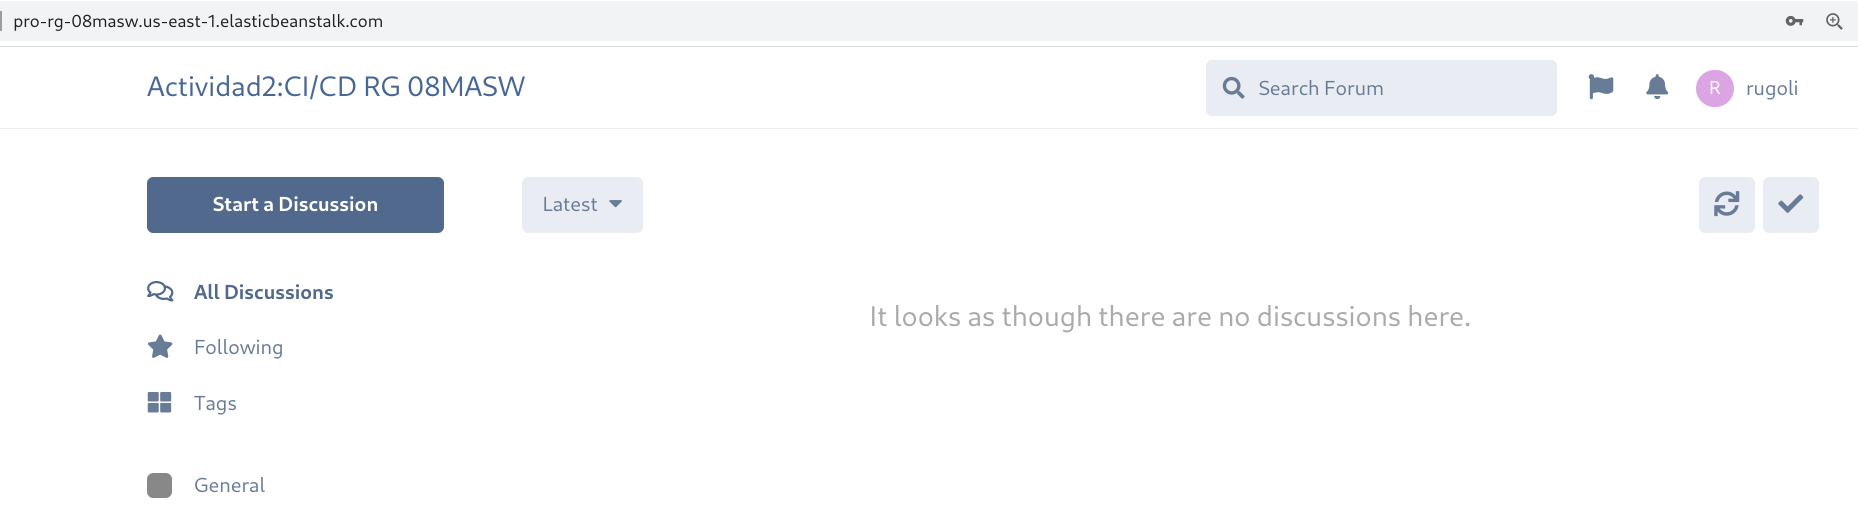
\includegraphics[frame,width=\linewidth]{img/flarum-3.png}
\end{center}

\chapter{IaC con Terraform}
\href{https://www.terraform.io/}{Terraform} es una aplicación que nos permite  la creación de toda la infraestructura dentro de una nube pública mediante código (IaC, \textit{Infraestructure as code}). De esta manera, podremos realizar despliegues automatizados para distintos entornos (desarrollo, test, producción...).

Para poder utilizar Terraform, una vez \href{https://developer.hashicorp.com/terraform/downloads}{descargado el binario}, tenemos que crear unas variables de entorno (con datos obtenidos de nuestra cuenta AWS) para que la conexión se realice de manera correcta y autenticada.

\begin{mycode}{Seteamos las variables de entorno}{console}{}
ruben@vega:~$ export AWS_ACCESS_KEY_ID=ASIAUSUHSKXGC...
ruben@vega:~$ export AWS_SECRET_ACCESS_KEY=iaC2DxU6Gg...
\end{mycode}

El siguiente paso es decidir qué queremos desplegar. Para esta prueba se va a desplegar una instancia RDS de MySQL similar a la del primer capítulo. Las característcas son:

\begin{itemize}
    \item RDS MySQL versión 5.7.X
    \item \textbf{Identificador RDS}: actividad2-terra
    \textbf{Nombre bd} = DB\_terra
    \textbf{User} = admTerra
    \textbf{Password} = Viu2022Terra
    \item \textbf{Tipo de instancia}: T3.micro
    \item \textbf{Tamaño}: 15GB
    \item \textbf{Periodo de retención backups}: 15 días
    \item \textbf{Hora de realización backups}: 03:00 UTC.
    \item \textbf{Ventana de mantenimiento}: 05:00 UTC
    \item \textbf{Cifrado activo}
\end{itemize}

Para realizar el despliegue tenemos que crear un fichero \configfile{main.tf} que contendrá las directivas que Terraform utilizará para conectarse a AWS y realizar el despliegue con las características previas.

\begin{mycode}{Fichero main.tf}{terraform}{}
terraform {
    required_providers {
        aws = {
            source  = "hashicorp/aws"
            version = "~> 4.16"
        }
    }
    required_version = ">= 1.2.0"
}
provider "aws" {
    region = "us-east-1"
}
resource "aws_db_instance" "actividad2-terra" {
    identifier              = "actividad2-terra"
    allocated_storage       = 15
    db_name                 = "DB_terra"
    engine                  = "mysql"
    engine_version          = "5.7"
    instance_class          = "db.t3.micro"
    username                = "admTerra"
    password                = "Viu2022Terra"
    parameter_group_name    = "default.mysql5.7"
    skip_final_snapshot     = true
    backup_retention_period = 15
    backup_window           = "03:00-03:30"
    maintenance_window      = "Sat:05:00-Sat:05:30"
    storage_encrypted       = true
}
\end{mycode}

Para asegurarnos que el fichero está bien creado, podemos ejecutar \commandbox{terraform validate}, después inicializar el entorno y aplicar los cambios que se van a realizar ya en AWS.

\begin{mycode}{Validar la configuración, inicializar y aplicar cambios}{console}{}
ruben@vega:~$ terraform validate
Success! The configuration is valid.

ruben@vega:~$ terraform init
Initializing the backend...
Initializing provider plugins...
- Finding hashicorp/aws versions matching "~> 4.16"...
- Installing hashicorp/aws v4.52.0...
- Installed hashicorp/aws v4.52.0 (signed by HashiCorp)
...
Terraform has been successfully initialized!

ruben@vega:~$ terraform apply
Terraform used the selected providers to generate the following
execution plan. Resource actions are indicated with the following
symbols:
+ create
Terraform will perform the following actions:
# aws_db_instance.actividad2-terra will be created
+ resource "aws_db_instance" "actividad2-terra" {
    + address                               = (known after apply)
    + allocated_storage                     = 15
...
}
Plan: 1 to add, 0 to change, 0 to destroy.

Do you want to perform these actions?
Terraform will perform the actions described above.
Only 'yes' will be accepted to approve.
  Enter a value: yes

aws_db_instance.actividad2-terra: Creating...
aws_db_instance.actividad2-terra: Still creating... [10s elapsed]
...
aws_db_instance.actividad2-terra: Creation complete
  after 9m15s [id=actividad2-terra]
Apply complete! Resources: 1 added, 0 changed, 0 destroyed.
\end{mycode}

Tras esperar unos minutos, el proceso termina, y desde el interfaz web ya podemos ver que nos aparece la instancia, y al ir a mirar su configuración podemos ver los detalles configurados en el fichero \configfile{main.tf}:


\begin{center}
    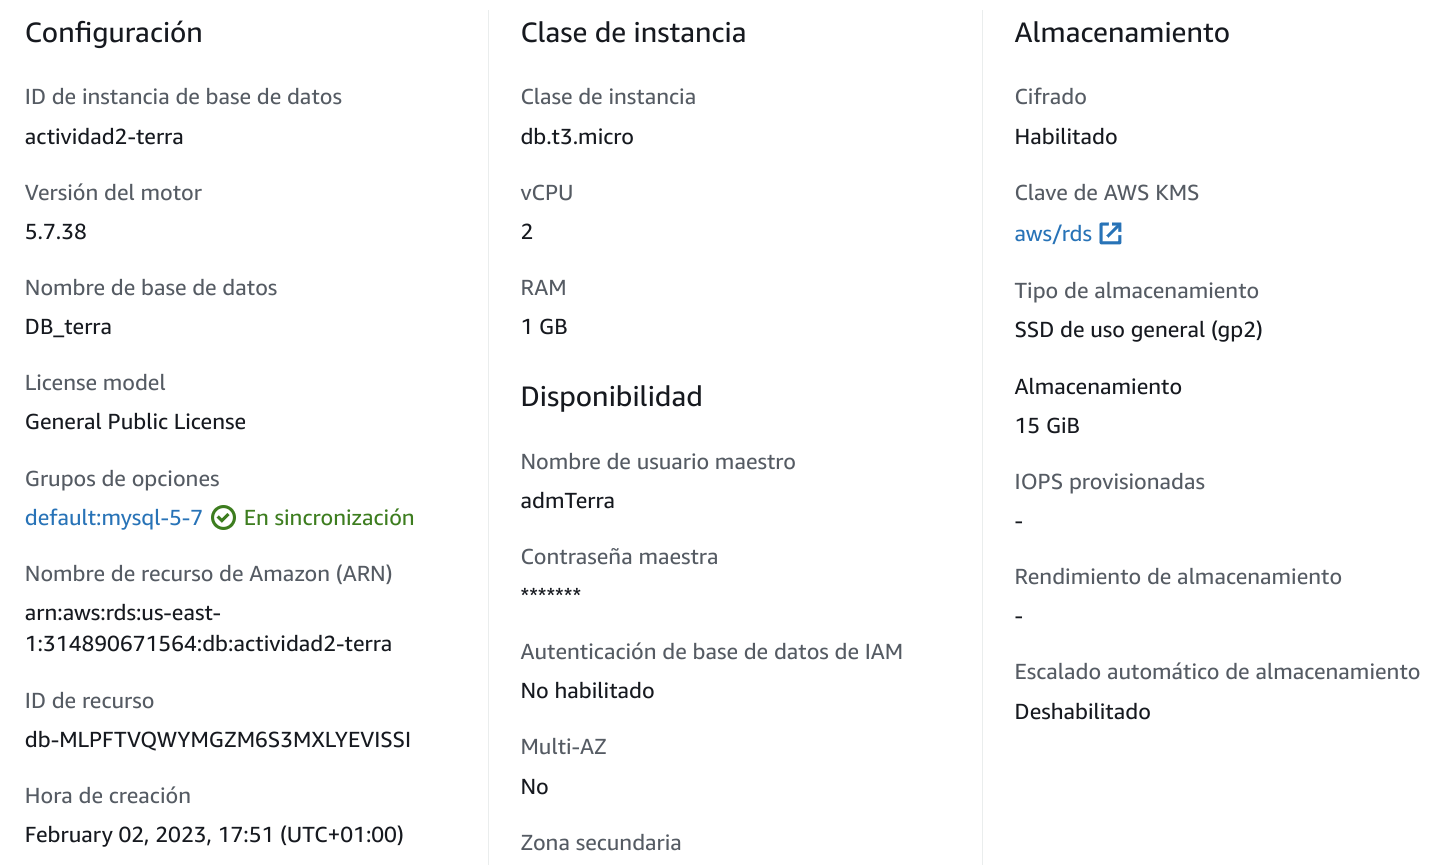
\includegraphics[frame,width=\linewidth]{img/terraform2.png}
\end{center}


En la siguiente imagen se puede comprobar cómo la instancia está funcionando:
\begin{center}
    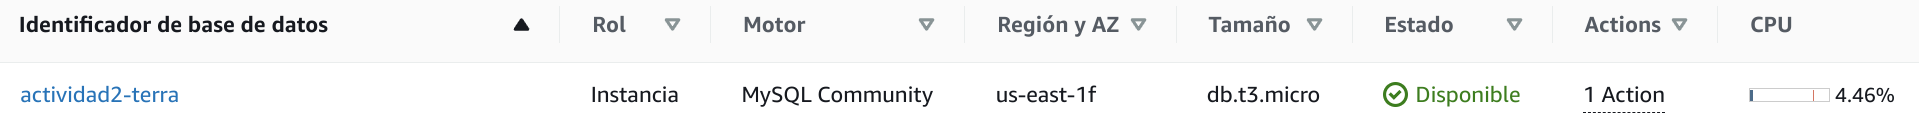
\includegraphics[frame,width=\linewidth]{img/terraform1.png}
\end{center}

Si nos interesase destruir la instancia de base de datos recién levantada, podríamos hacerlo con \commandbox{terraform destroy}, y comenzaría con el proceso de parada y eliminación.

\chapter{Conclusiones}

La automatización del despliegue de aplicaciones, a través de sistemas CI/CD como el que ofrece GitlLab, nos va a permitir que una vez creado el proceso podamos replicarlo tantas veces como sea necesario. De esta manera, podremos utilizarlo para realizar pases a producción, evitando tener que repetir cada vez el proceso y así evitar posibles olvidos o fallos durante el proceso.

Si esto mismo lo utilizamos para realizar despliegues a nivel de infraestructura con Terraform, podremos realizar despliegues enteros para distintos entornos asegurando que no existen diferencias entre ellos.

Tal como se puede ver, cuando vayamos a utilizar una infraestructura \textit{Cloud}, es obligatorio hacer uso de las herramientas que nos van a permitir realizar un trabajo repetitivo de manera más eficiente y segura.

\end{document}
